\begin{center}

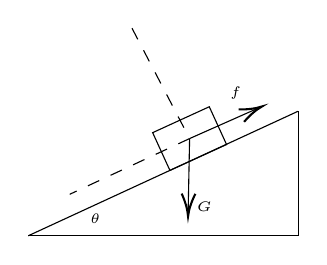
\begin{tikzpicture}[x=0.75pt,y=0.75pt,yscale=-1,xscale=1]
%uncomment if require: \path (0,300); %set diagram left start at 0, and has height of 300

%Straight Lines [id:da9008116307778782] 
\draw    (200,200) -- (330,140) ;
%Shape: Rectangle [id:dp03770706202210139] 
\draw   (259.95,150.31) -- (287.23,137.83) -- (295.55,156.02) -- (268.26,168.5) -- cycle ;
%Straight Lines [id:da8341542863429008] 
\draw    (200,200) -- (330,200) ;
%Straight Lines [id:da1419286936694566] 
\draw    (330,140) -- (330,200) ;
%Straight Lines [id:da8505072201094237] 
\draw  [dash pattern={on 4.5pt off 4.5pt}]  (277.75,153.16) -- (220,180) ;
%Straight Lines [id:da9138661314002989] 
\draw  [dash pattern={on 4.5pt off 4.5pt}]  (250,100) -- (277.75,153.16) ;
%Straight Lines [id:da2057884653890707] 
\draw    (277.75,153.16) -- (277.04,188.67) ;
\draw [shift={(277,190.67)}, rotate = 271.14] [color={rgb, 255:red, 0; green, 0; blue, 0 }  ][line width=0.75]    (10.93,-3.29) .. controls (6.95,-1.4) and (3.31,-0.3) .. (0,0) .. controls (3.31,0.3) and (6.95,1.4) .. (10.93,3.29)   ;
%Straight Lines [id:da1801333502686453] 
\draw    (277.75,153.16) -- (310.84,138.48) ;
\draw [shift={(312.67,137.67)}, rotate = 156.07] [color={rgb, 255:red, 0; green, 0; blue, 0 }  ][line width=0.75]    (10.93,-3.29) .. controls (6.95,-1.4) and (3.31,-0.3) .. (0,0) .. controls (3.31,0.3) and (6.95,1.4) .. (10.93,3.29)   ;

% Text Node
\draw (280,182.33) node [anchor=north west][inner sep=0.75pt]  [font=\tiny] [align=left] {$\displaystyle G$};
% Text Node
\draw (296,127) node [anchor=north west][inner sep=0.75pt]  [font=\tiny] [align=left] {$\displaystyle f$};
% Text Node
\draw (228.67,188) node [anchor=north west][inner sep=0.75pt]  [font=\tiny] [align=left] {$\displaystyle \theta $};


\end{tikzpicture}

\end{center}